\chapter{Design}
\label{design}

\section{Introduction}

\section{Framework Design}

Spring MVC and Hibernate incorporates a number of design patterns within its own classes. By using these frameworks, developers are guided towards best practice in terms of the application design

\begin{table}[H]
\begin{enumerate}
\item Singleton
\begin{itemize}
\item Beans defined within the Spring MVC framework and singletons by default. 
\end{itemize}
\item Factory
\begin{itemize}
\item The Factory pattern is used for loading Beans through the \textit{BeanFactory} class, and the \textit{Application Context}. 
\end{itemize}
\item Inversion of Control
\begin{itemize}
\item This pattern is central to the dependency injection facilities of the Spring framework, and is responsible for the instantiation of objects at run time, rather than compile time.
\end{itemize}
\item Query Object
\begin{itemize}
\item This pattern is used by Hibernate with its Criterion object. This delegates the execution of a query to another object. 
\end{itemize}
\end{enumerate}
\label{fig:springdesignpatterns}
\end{table}

\label{sec:design}
\section{Controller-Service-DAO Design}

In order to achieve modularity across the application, the core of the application is separated into four key areas.


\begin{enumerate}
\item Entities
\begin{itemize}
\item A Java object that is persisted to a table in a relational database.
\end{itemize}
\item Controllers
\begin{itemize}
\item A controller will handled the user requests the application must deal with
\end{itemize}
\item Service
\begin{itemize}
\item The Service layer facilitates communication between the controller and the DAO layer.
\end{itemize}
\item Data Access Objects [DAO]
\begin{itemize}
\item This layer is responsible for persisting an entity or any changes to an entity.
\end{itemize}
\end{enumerate}
\begin{figure}[H]
\label{fig:appbreakdown}
\end{figure}

This structure follows a design principle called \textit{Separation of Concerns}. This separates an application into a number of component parts in order to minimise the effect that changes in one module have on other modules. In this application, any changes to the DAO layer will have no effect on the Controller layer for example. This is realised through this design principle, and the use of the Hibernate framework.

The flow between these objects is shown in Figure~\ref{fig:csdao}. An example flow would be the creation of a user objects. 

\begin{figure}[H]
\begin{center}
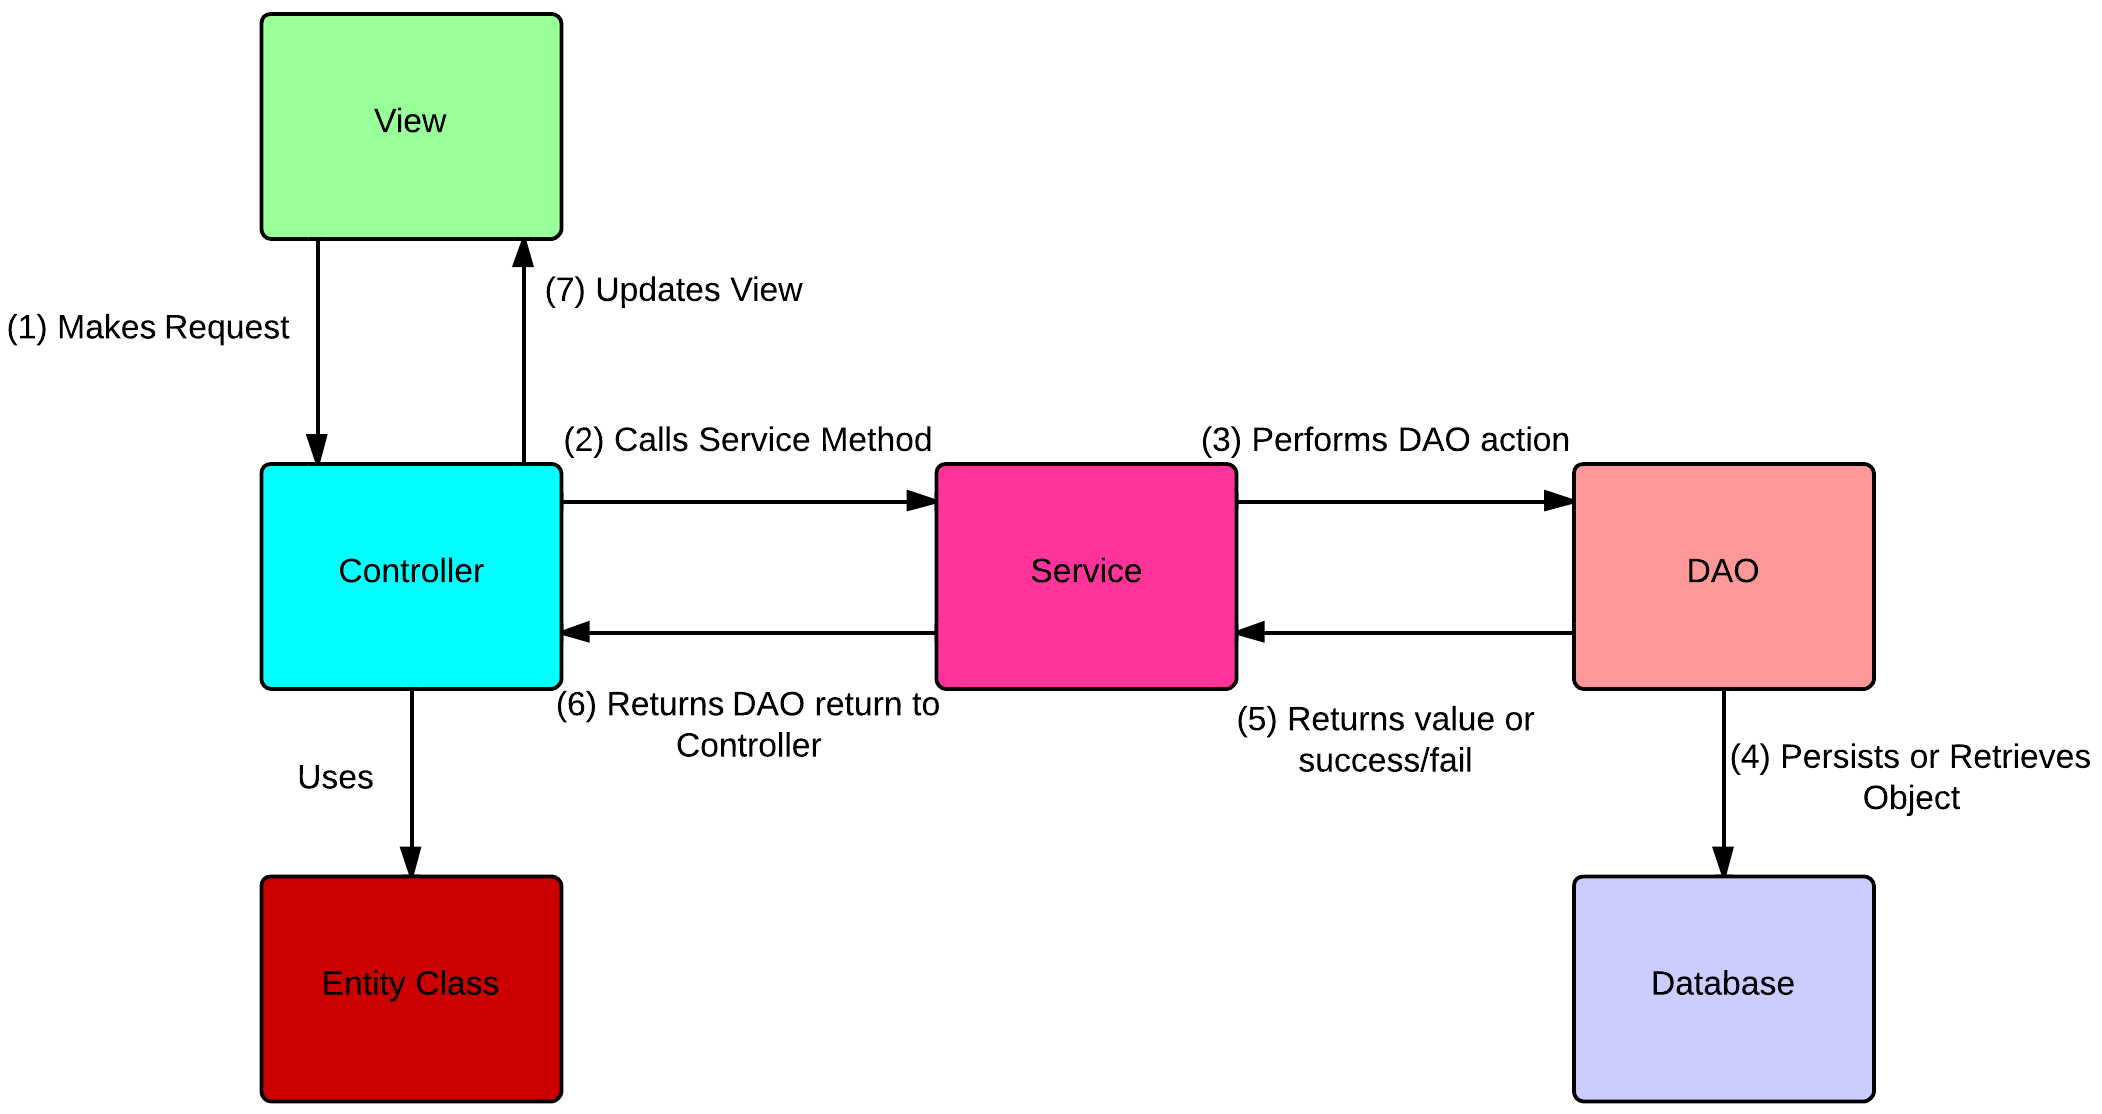
\includegraphics[width=14cm]{csdao.png}
\end{center}
\caption{Controller-Service-DAO Flow}
\label{fig:csdao}
\end{figure}

\subsection{User Roles}

The User class was designed with the existing application form of Monaleen Tennis Club as a foundation. 
Spring controls access within the application. Firstly, it uses an \textit{authority} hierarchy to separate different levels of users. For this web application, there were three main levels of authority, with one level containing three different branches.

\subsubsection{Roles}
\begin{itemize}
\item ROLE ADMIN
\begin{itemize}
\item This refers to the main administration group. The group retains full rights across the web application
\end{itemize}
\item ROLE COMMITTEE
\begin{itemize}
\item This refers to the committee, as defined by the club themselves. This group with have the ability to perform some administrator privileges, but only those directly related to club activities, not site activities.
\end{itemize}
\item ROLE MEMBER
\begin{itemize}
\item The default user state. This group can perform actions such as booking slots in a timetable, registering for a tournament, and will have access to parts of the site unavailable to non-registered users.
\end{itemize}
\item ROLE WARNING 
\begin{itemize}
\item A restriction placed upon a member. For example, a member who books time slots, but does not attend. In this application, it reduces the number of allowed bookings on a court per week from 3 to 2.
\end{itemize}
\item ROLE SUSPEND
\begin{itemize}
\item A further restriction placed upon a member. Number of bookings on a court per week reduced to 1.
\end{itemize}
\end{itemize}
\label{fig:secRoles}


\subsection{Database Design}

The database was designed using MySQL Workbench, and created using the same tool. The database Entity Relationship (ER) diagram is illustrated in Figure~\ref{fig:dbdesign}

\begin{figure}[H]
\begin{center}
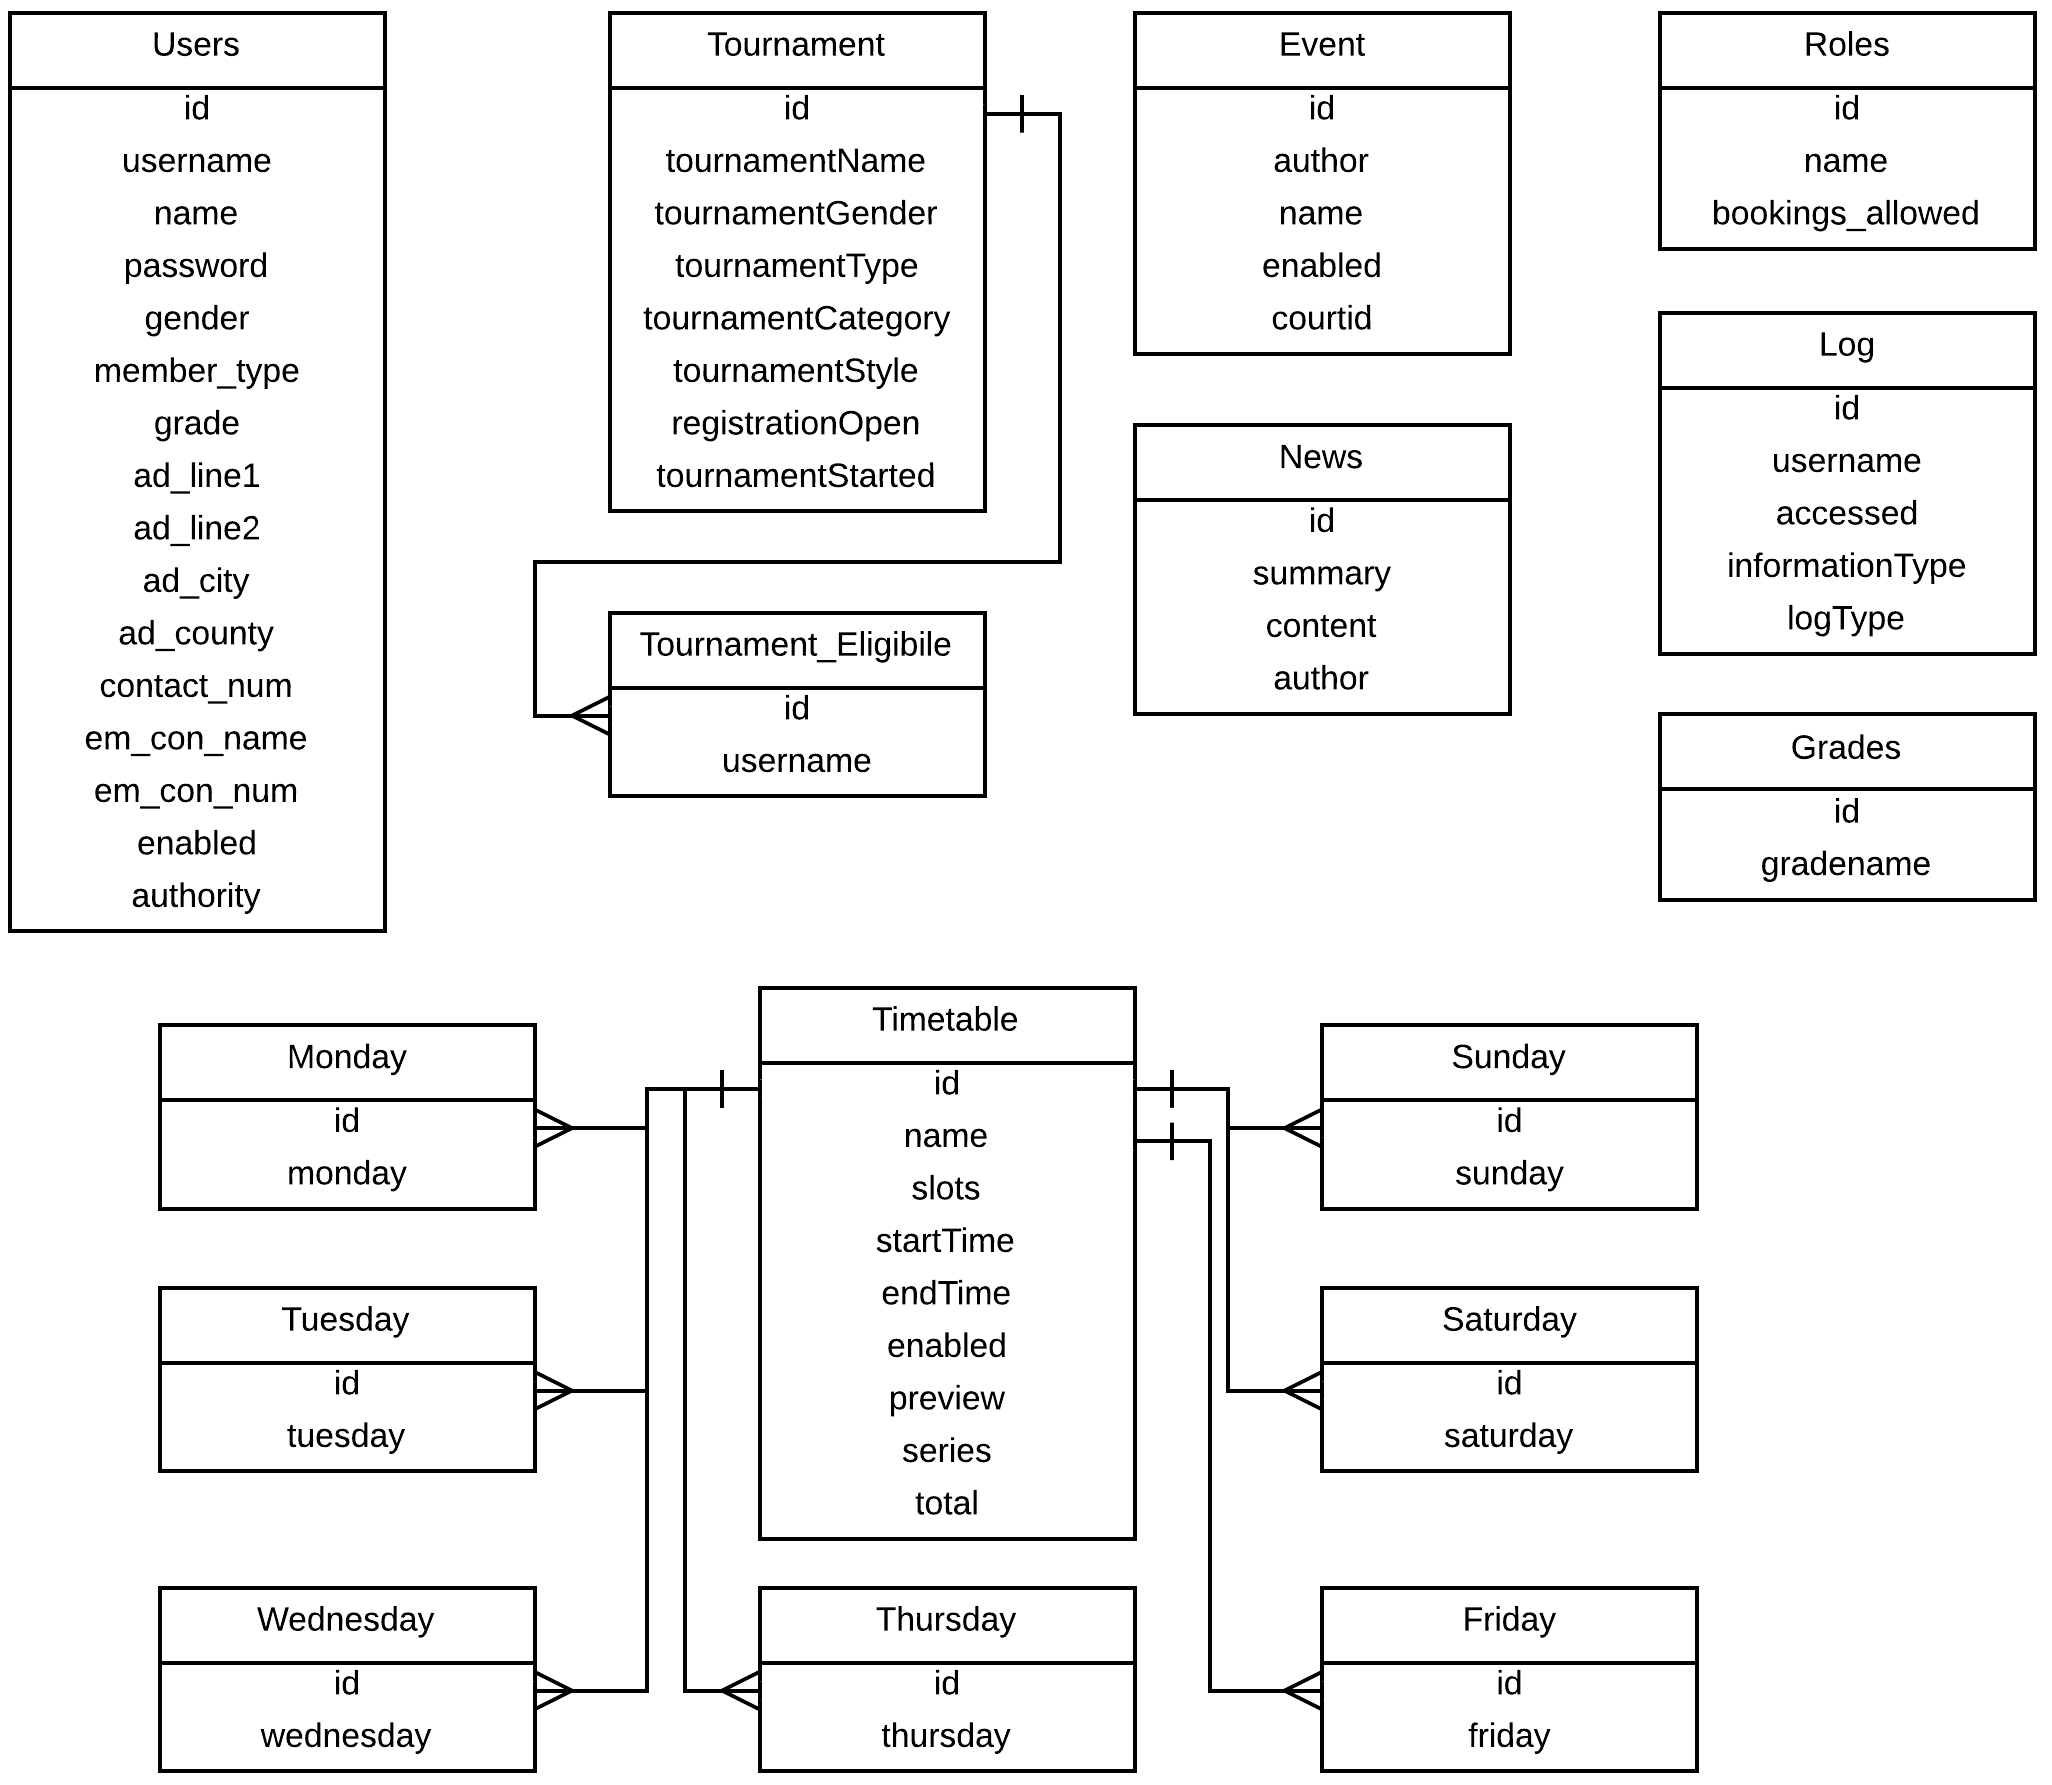
\includegraphics[width=14cm]{dbdesign.png}
\end{center}
\caption{Database Design}
\label{fig:dbdesign}
\end{figure}

